
\chapter{Pitch angle threshold}\label{a1}

\begin{figure}
    \centering
    \begin{subfigure}[t]{.5\textwidth}
        \centering
        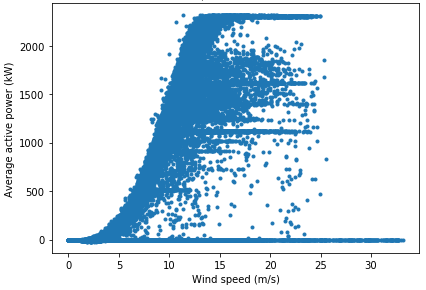
\includegraphics[height=5cm]{fa1a}
        \caption{}
    \end{subfigure}%
    \begin{subfigure}[t]{.5\textwidth}
        \centering
        
\includegraphics[height=5cm]{fa1b}
        \caption{}
    \end{subfigure}
    \begin{subfigure}[t]{.49\textwidth}
        \centering
        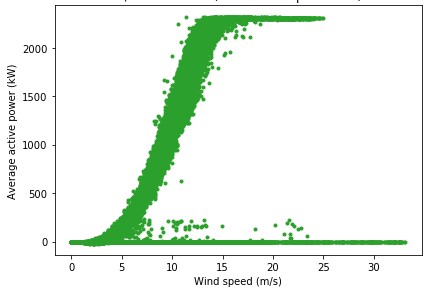
\includegraphics[height=5cm]{fa1c}
        \caption{}
    \end{subfigure}
    \begin{subfigure}[t]{.49\textwidth}
        \centering
        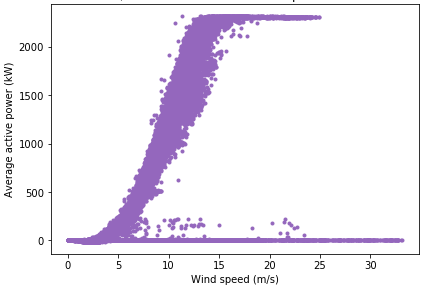
\includegraphics[height=5cm]{fa1d}
        \caption{}
    \end{subfigure}
    \captionsetup{labelformat=empty,list=no}
    \caption{Power curves for turbine 1 used in selecting the pitch angle threshold. a is the original power curve. In b, data points with a pitch angle not equal to 0\,\textdegree between 90\,\% and 10\,\% power were filtered out, which distorts the power curve shape. In c, all data points have a pitch angle between 0\,\textdegree and 3.5\,\textdegree, which removes most curtailment and anomalous points while maintaining the typical power curve shape. In d, all data points have a pitch angle between 0\,\textdegree and 7\,\textdegree, which allows some curtailment points to appear. Therefore, it was decided that the filter used in c is the most suitable.}
\end{figure}

\chapter{Power before cut-in threshold}\label{a2}

\begin{figure}
    \centering
    \begin{subfigure}[t]{.5\textwidth}
        \centering
        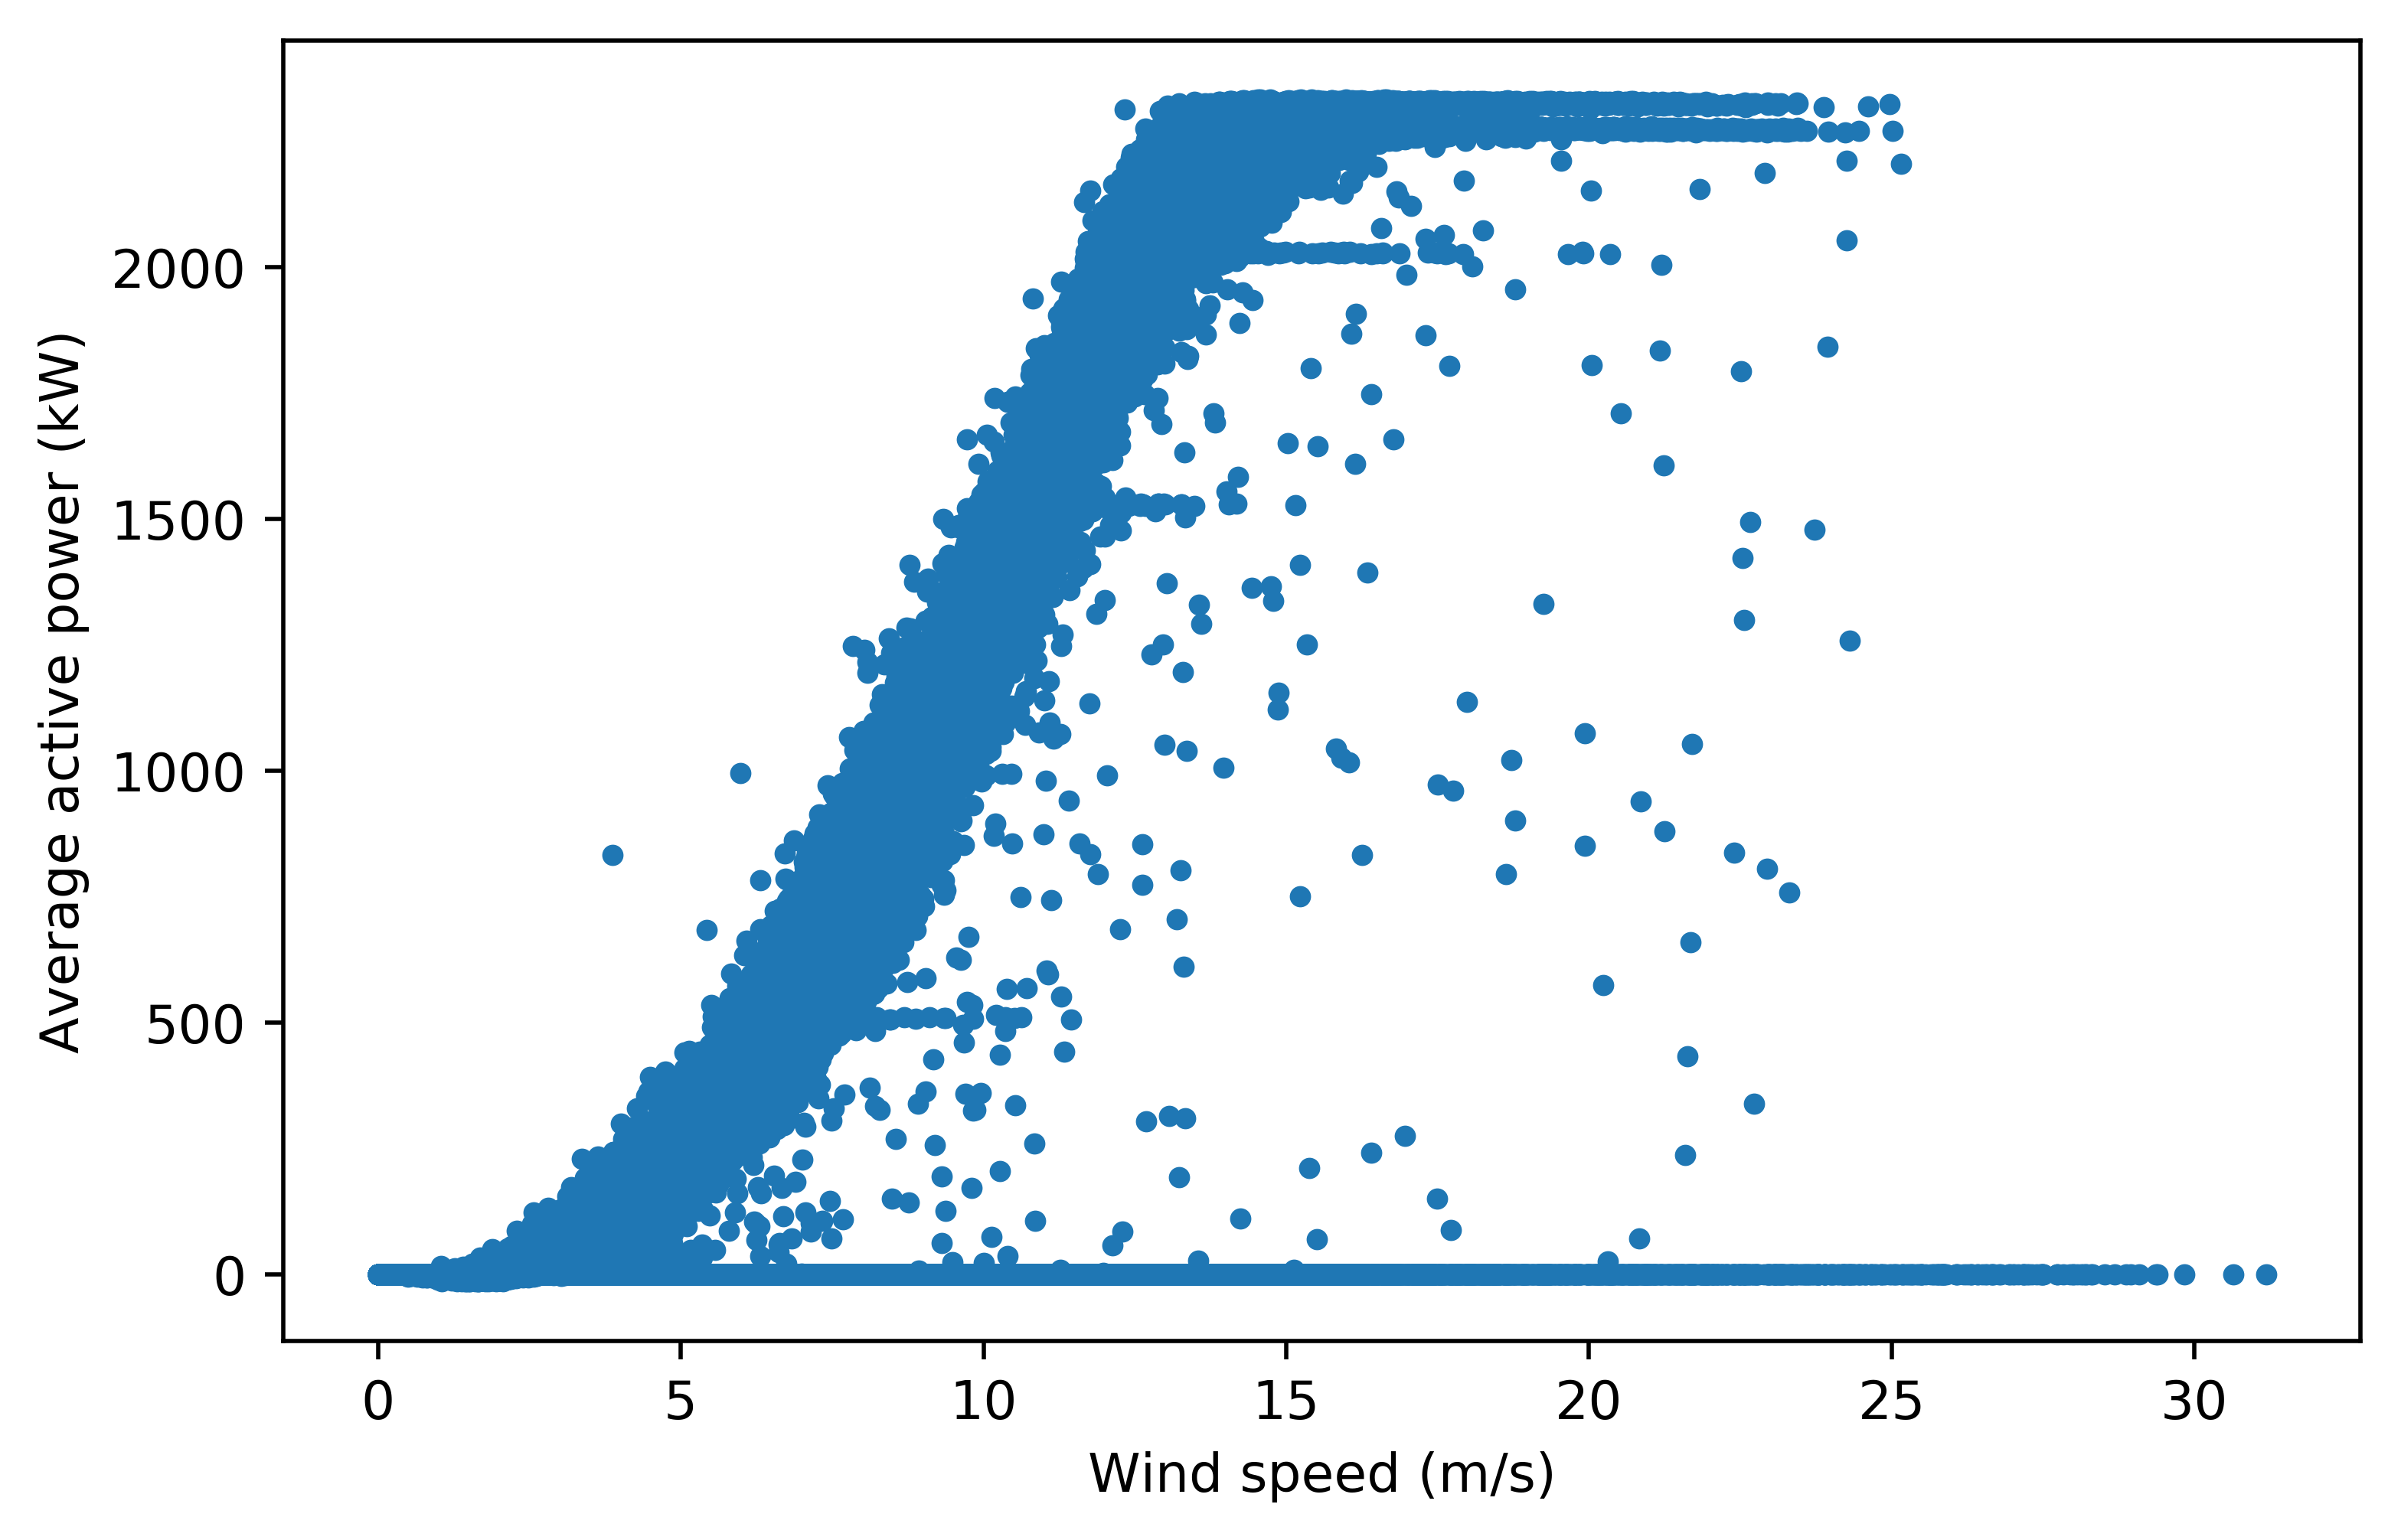
\includegraphics[height=5cm]{fa2a}
        \caption{}
    \end{subfigure}%
    \begin{subfigure}[t]{.5\textwidth}
        \centering
        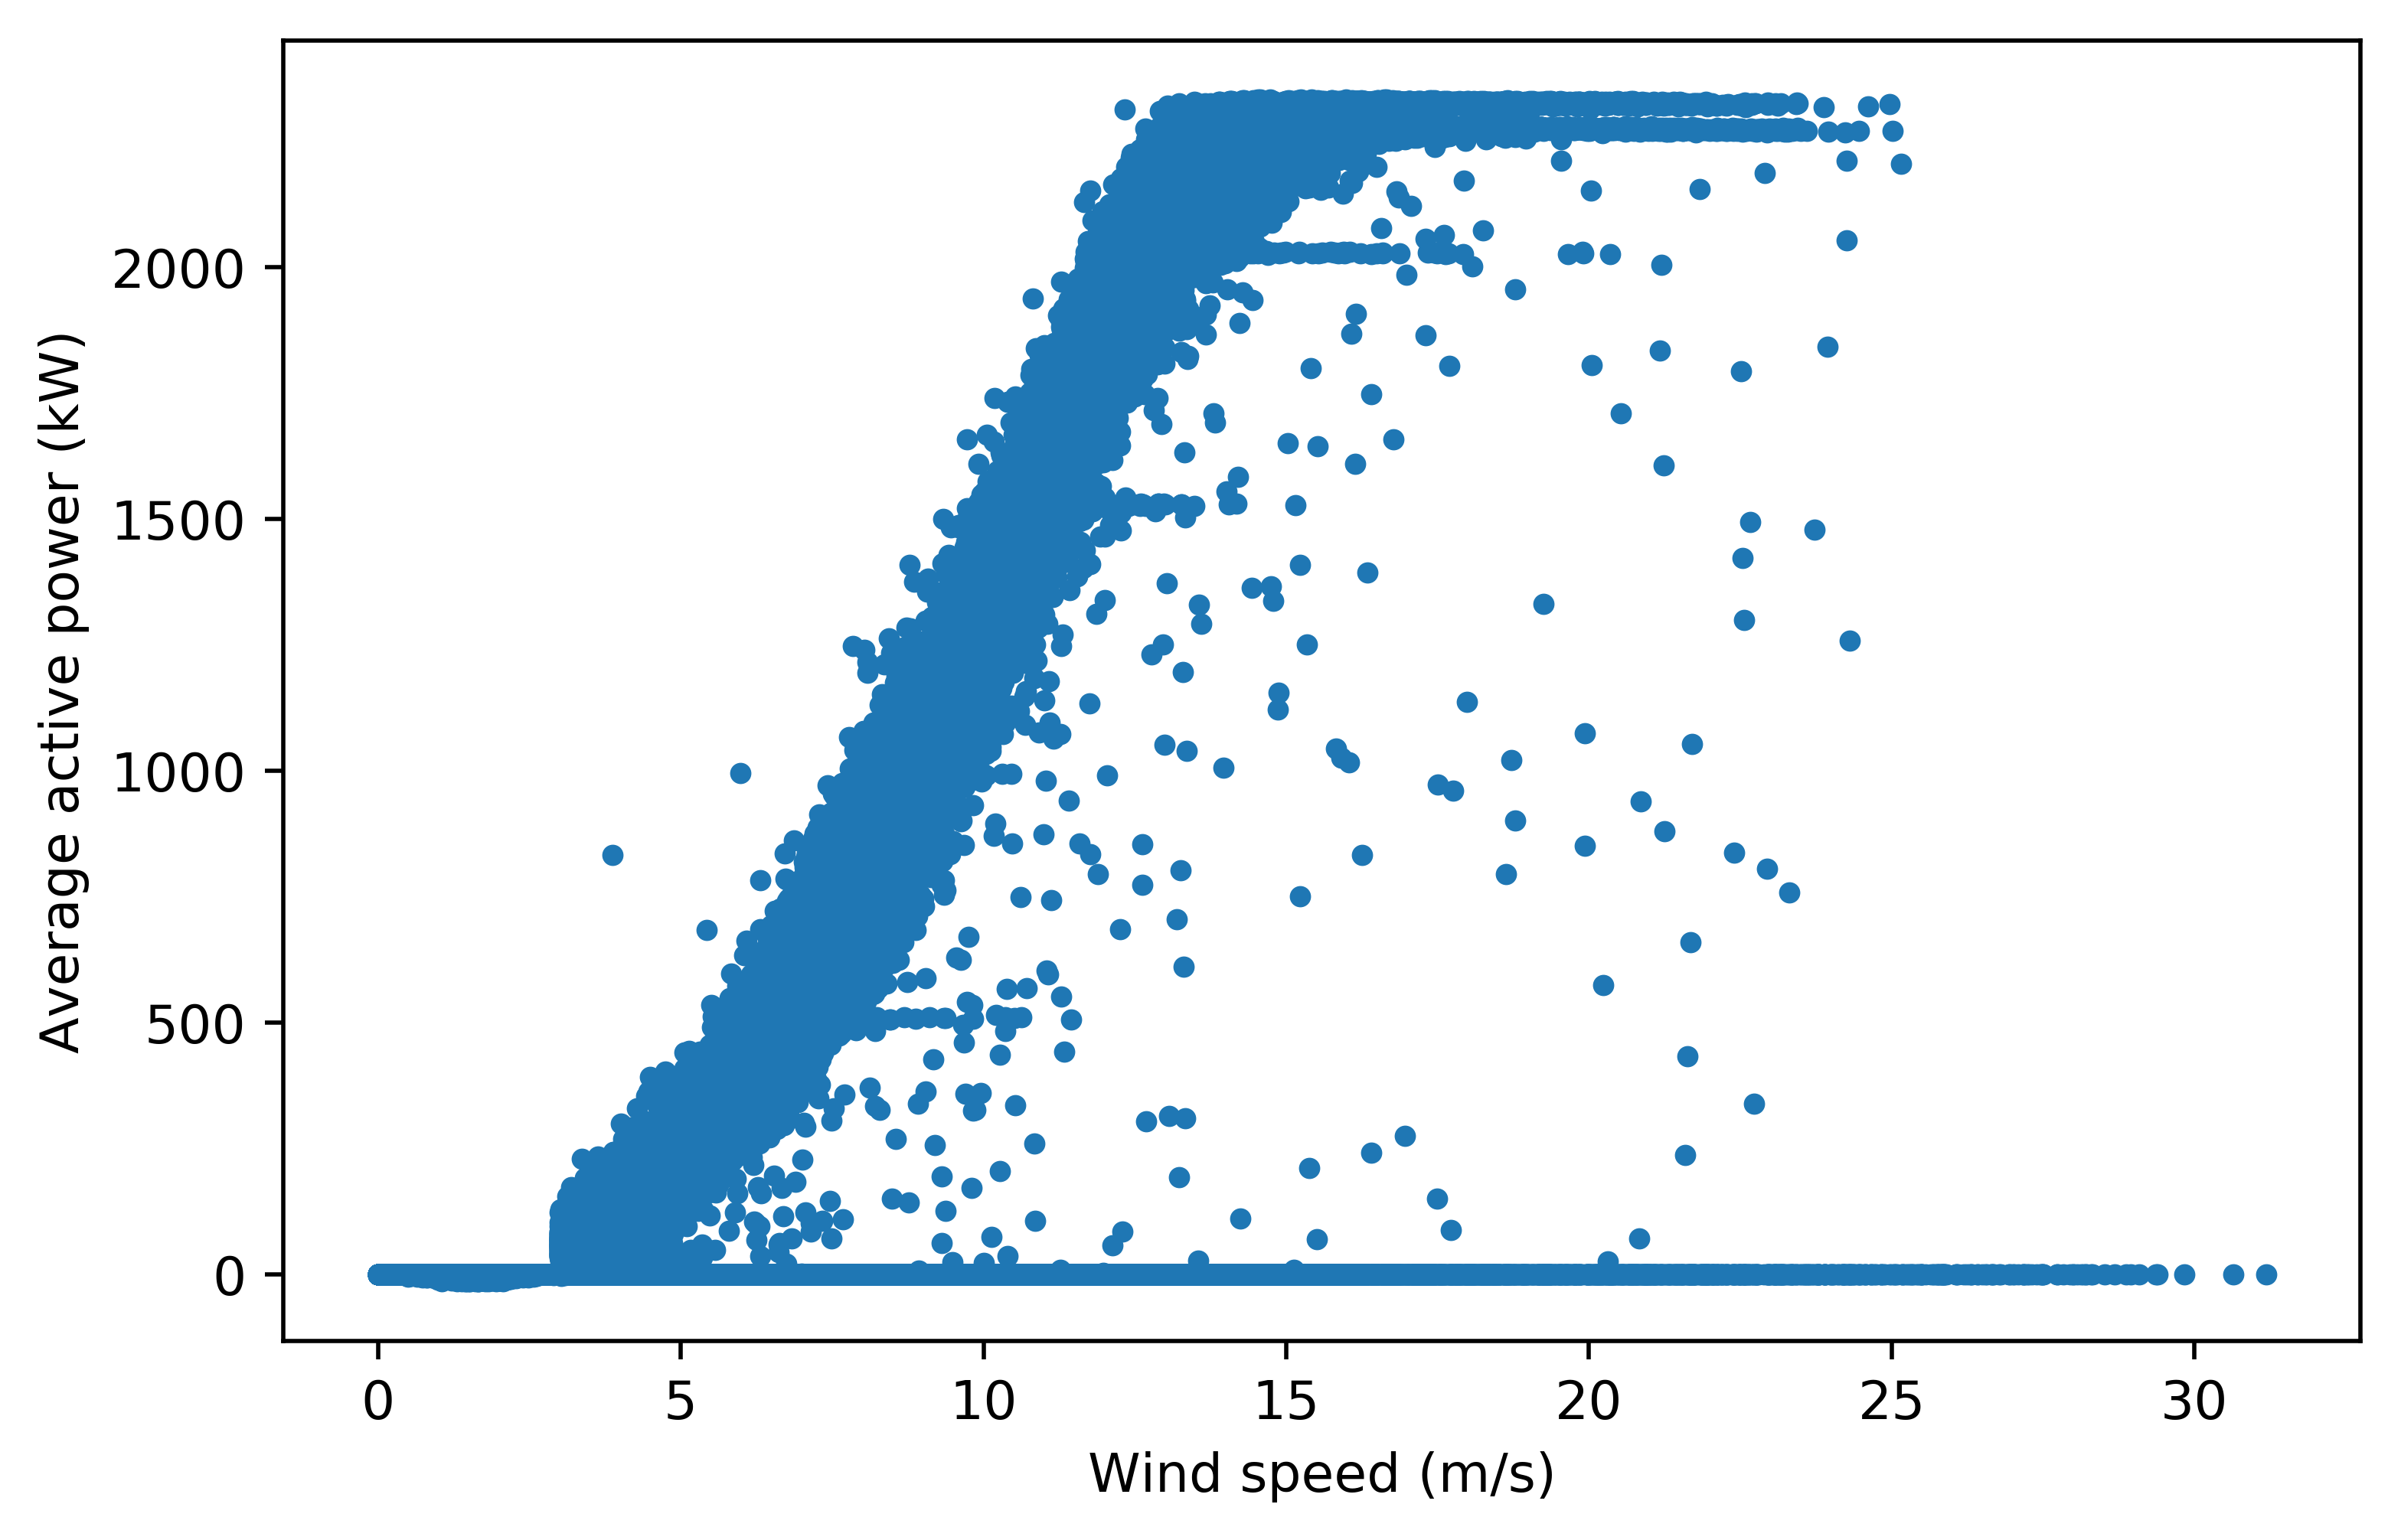
\includegraphics[height=5cm]{fa2b}
        \caption{}
    \end{subfigure}
    \captionsetup{labelformat=empty,list=no}
    \caption{Power curves for turbine 24 used in selecting the power threshold before cut-in speed. a is the original power curve. b is the power curve with a filter applied to remove all data points with power > 0 kW before the cut-in speed of 3 m/s. Anemometer wind speeds, which were used to plot these power curves, are not an accurate measure of the wind speed incident on the turbine blades. Therefore, a threshold of 100 kW before cut-in is applied, which maintains the power curve shape for all 25 turbines while removing anomalous points, such as the ones in turbine 2's power curve.}
\end{figure}

\chapter{Results for random forest classifier}\label{a3}

\begin{landscape}
    \begin{table}
        \centering
        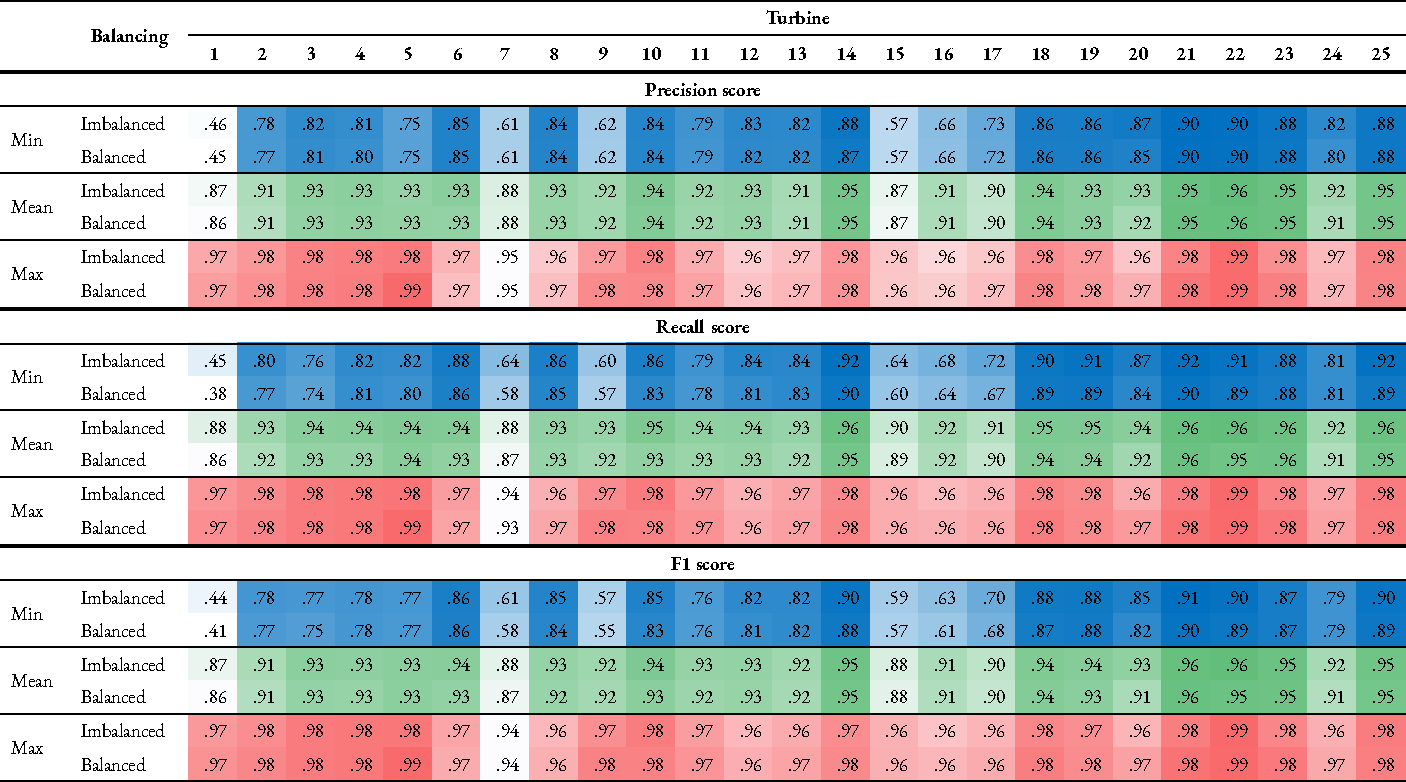
\includegraphics{ta1}
        \captionsetup{labelformat=empty,list=no}
        \caption{Precision, recall and F1 scores for each turbine using random forest classifier for both imbalanced and balanced training data. The table lists the minimum, mean and maximum values for each score, which are also colour-coded to show higher scores in darker shades and lower scores in lighter shades.}
    \end{table}
\end{landscape}

\begin{table}
    \centering
    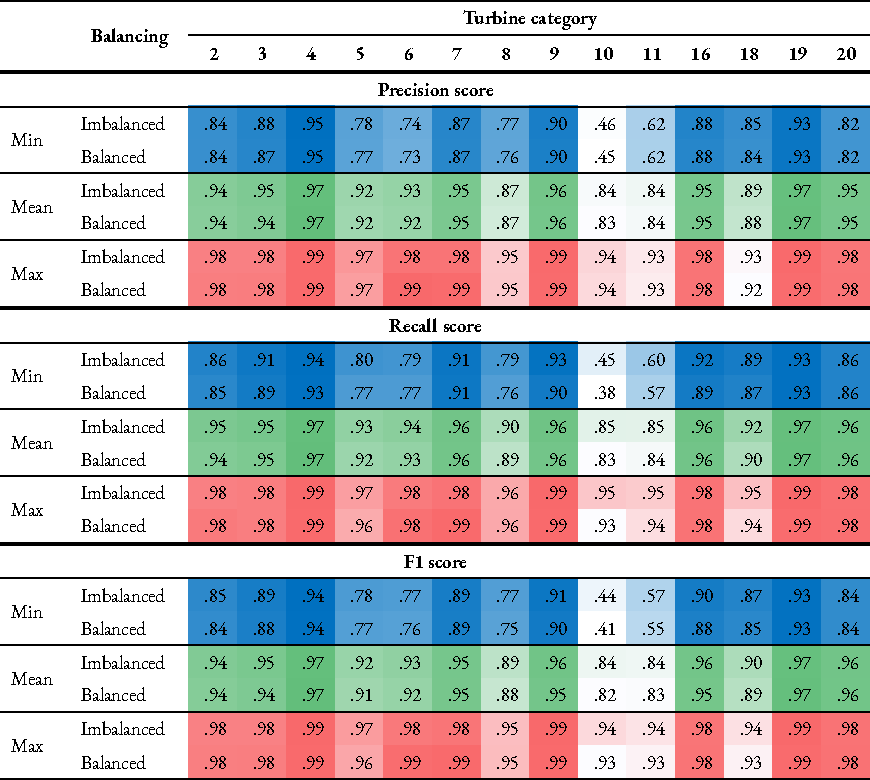
\includegraphics{ta2}
    \captionsetup{labelformat=empty,list=no}
    \caption{Precision, recall and F1 scores for each turbine category using random forest classifier for both imbalanced and balanced training data. The table lists the minimum, mean and maximum values for each score, which are also colour-coded to show higher scores in darker shades and lower scores in lighter shades.}
\end{table}

\chapter{Confusion matrices}\label{a4}

\begin{table}
    \centering
    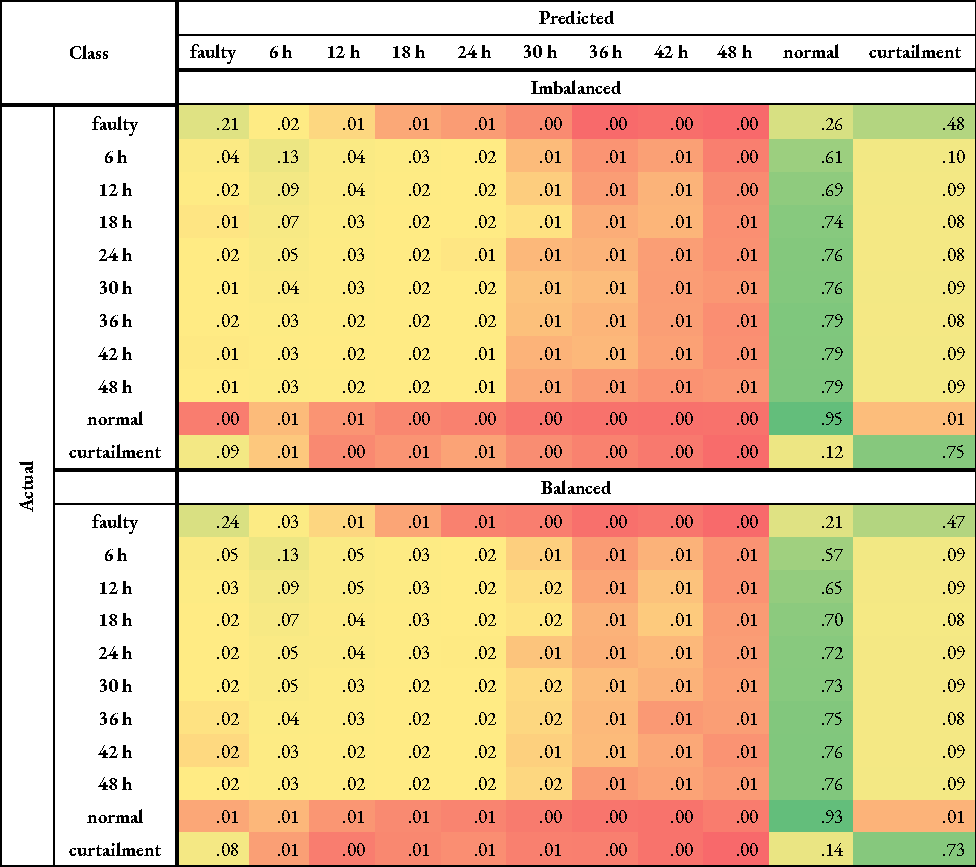
\includegraphics[width=.99\textwidth]{ta3}
    \captionsetup{labelformat=empty,list=no}
    \caption{Normalised confusion matrices for turbine category 10 (`electrical system') with all classes used in the classification process using random forests and either imbalanced or balanced training data. The matrix is colour-coded; it transitions from red (lower scores) to yellow (intermediate) to green (higher scores).}
\end{table}

\begin{table}
    \centering
    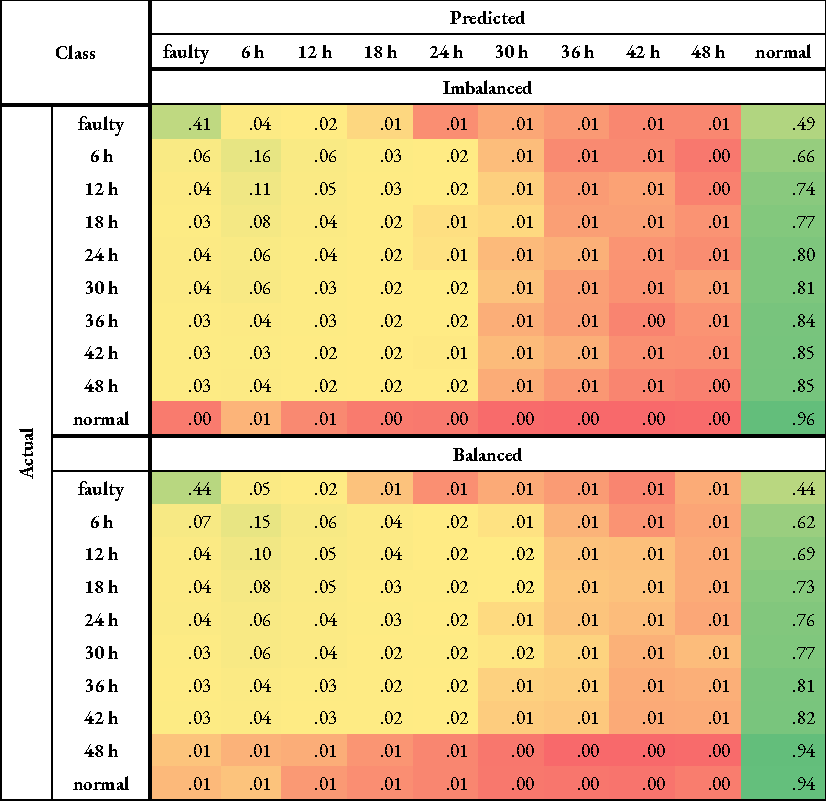
\includegraphics{ta4}
    \captionsetup{labelformat=empty,list=no}
    \caption{Normalised confusion matrices for turbine category 10 (`electrical system') when classification is done using random forests and either imbalanced or balanced training data without the `curtailment' class (i.e., rows of data with curtailment or anomalies in any label are dropped). The matrix is colour-coded, transitioning from red (lower scores) to yellow (intermediate) to green (higher scores).}
\end{table}

\begin{table}
    \centering
    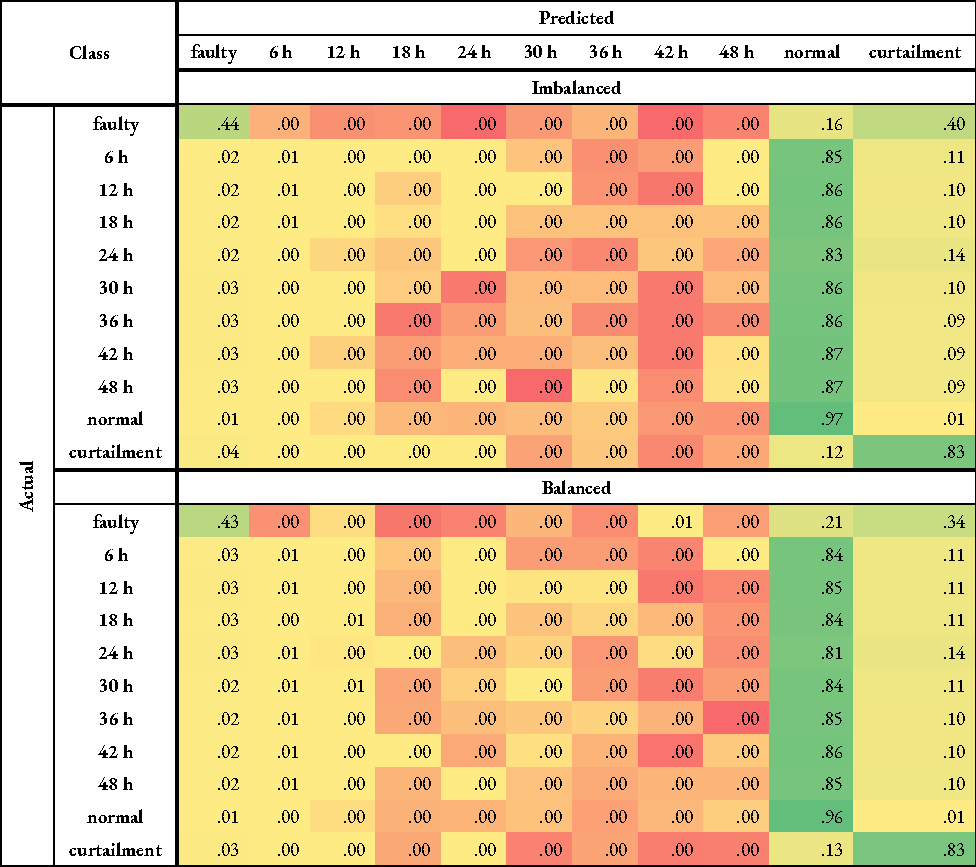
\includegraphics[width=.99\textwidth]{ta5}
    \captionsetup{labelformat=empty,list=no}
    \caption{Normalised confusion matrices for turbine category 5 (`gearbox') with all classes used in the classification process using random forests and either imbalanced or balanced training data. The matrix is colour-coded; it transitions from red (lower scores) to yellow (intermediate) to green (higher scores).}
\end{table}

\begin{table}
    \centering
    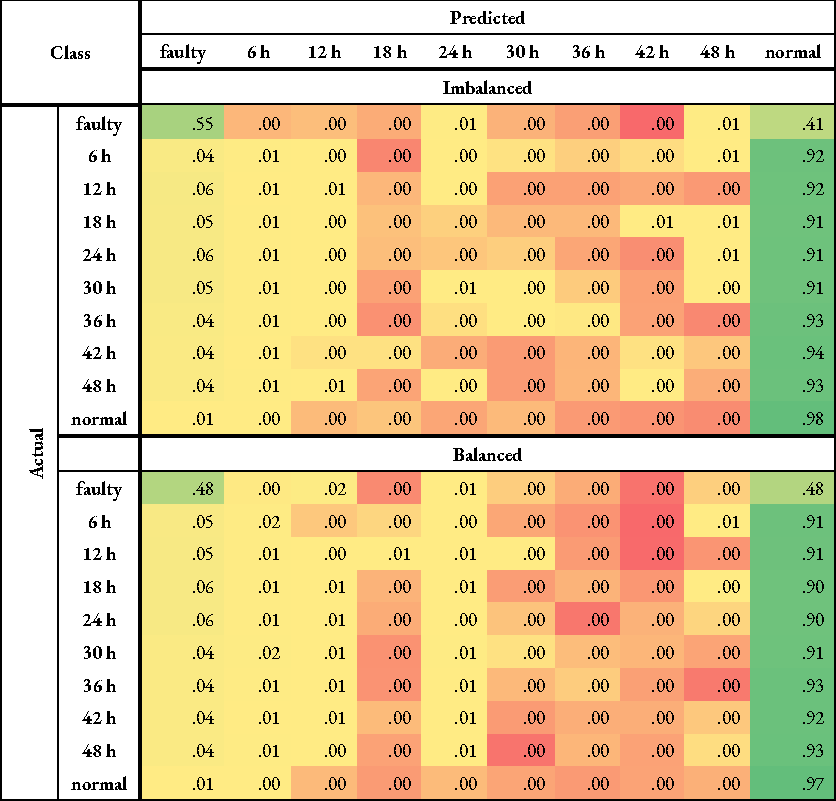
\includegraphics{ta6}
    \captionsetup{labelformat=empty,list=no}
    \caption{Normalised confusion matrices for turbine category 5 (`gearbox') when classification is done using random forests and either imbalanced or balanced training data without the `curtailment' class (i.e., rows of data with curtailment or anomalies in any label are dropped). The matrix is colour-coded, transitioning from red (lower scores) to yellow (intermediate) to green (higher scores).}
\end{table}

\chapter{Python codes}\label{a5}

Python codes used in this project can be found in its GitHub repository, which can be accessed through the following link: \url{https://github.com/nmstreethran/WindTurbineClassification}.
